% Standalone vector map of one shared Pythia/GPT-NeoX transformer block.
% Compile with:
%   pdflatex -interaction=nonstopmode -halt-on-error pythia-architecture-map.tex
% Manuscript inclusion:
%   
\includegraphics[width=\linewidth]{artifacts/pythia-architecture-map.pdf}
\documentclass[border=5pt]{standalone}

\usepackage{amsmath}
\usepackage{graphicx}
\usepackage{lmodern}
\usepackage{tikz}
\usepackage{xcolor}
\usetikzlibrary{arrows.meta,calc,positioning}

\definecolor{ink}{HTML}{203246}
\definecolor{muted}{HTML}{657483}
\definecolor{panelborder}{HTML}{A9B6C2}
\definecolor{panelfill}{HTML}{FBFCFD}
\definecolor{residualfill}{HTML}{294F63}
\definecolor{sitefill}{HTML}{E3F3ED}
\definecolor{siteborder}{HTML}{197A63}
\definecolor{weightfill}{HTML}{DCCEE8}
\definecolor{weightborder}{HTML}{76508F}
\definecolor{opfill}{HTML}{F1F3F5}
\definecolor{opborder}{HTML}{687581}

\tikzset{
  every node/.style={font=\sffamily\footnotesize, text=ink},
  flow/.style={-{Latex[length=2.0mm,width=1.25mm]}, draw=ink,
    line width=0.68pt, rounded corners=1.8pt},
  residualflow/.style={flow, line width=0.88pt},
  box/.style={rectangle, rounded corners=2.4pt, minimum height=6.2mm,
    align=center, inner xsep=4.0pt, inner ysep=1.8pt},
  site/.style={box, draw=siteborder, fill=sitefill, line width=0.82pt,
    font=\sffamily\bfseries\footnotesize, minimum width=7.2mm},
  weight/.style={box, draw=weightborder, fill=weightfill, line width=0.78pt,
    minimum width=9.0mm},
  op/.style={box, draw=opborder, fill=opfill, line width=0.58pt,
    minimum width=9.0mm},
  residual/.style={box, draw=residualfill, fill=residualfill, text=white,
    line width=0.72pt, font=\sffamily\bfseries\footnotesize,
    minimum width=10.0mm},
  merge/.style={box, draw=ink, fill=white, line width=0.82pt,
    minimum width=6.2mm, minimum height=6.2mm, inner sep=0pt,
    font=\sffamily\bfseries\normalsize},
  title/.style={font=\sffamily\bfseries\small, text=ink, inner sep=0pt},
  lane/.style={font=\sffamily\bfseries\scriptsize, text=muted},
  sublabel/.style={font=\sffamily\tiny, text=muted, align=center},
  keytext/.style={font=\sffamily\scriptsize, text=ink, inner sep=0pt},
  keydot/.style={circle, minimum size=2.6mm, inner sep=0pt, draw=none}
}
\newsavebox{\diagrambox}

\begin{document}
\global\pdfpageattr{/Rotate 90}% explicit viewer rotation for horizontal presentation
\begin{lrbox}{\diagrambox}
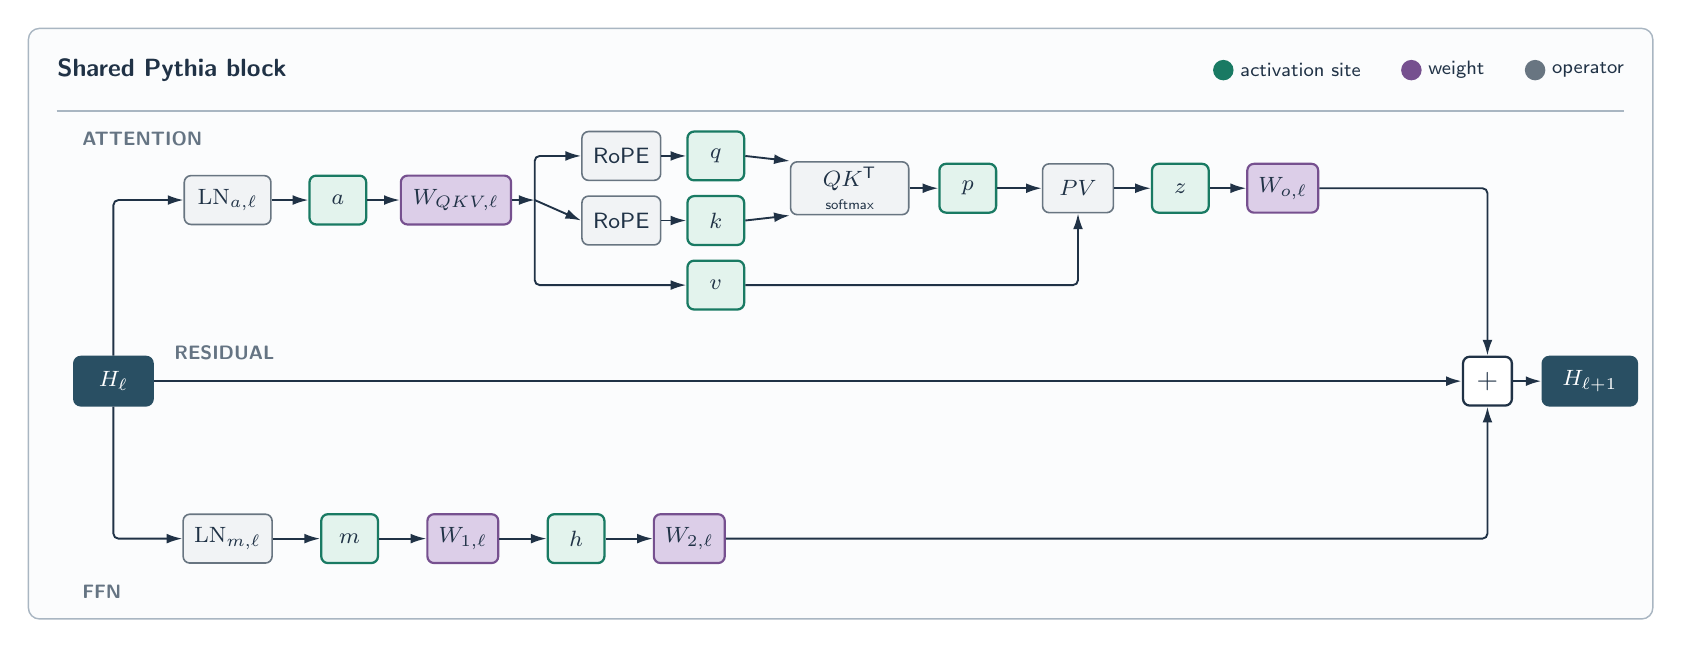
\begin{tikzpicture}[x=1cm,y=1cm]
  % One enclosing panel keeps the figure visually self-contained.
  \draw[draw=panelborder, fill=panelfill, line width=0.52pt, rounded corners=4pt]
    (-0.18,-3.02) rectangle (20.45,4.48);
  \draw[draw=panelborder, line width=0.42pt] (0.18,3.43) -- (20.09,3.43);

  % Header and compact, self-labeling semantic key.
  \node[title, anchor=west] at (0.18,3.95)
    {Shared Pythia block};
  \node[keytext, anchor=east] (operator-key) at (20.09,3.95) {operator};
  \node[keydot, fill=opborder] (operator-dot)
    at ([xshift=-2.1mm]operator-key.west) {};
  \node[keytext, anchor=east] (weight-key)
    at ([xshift=-5mm]operator-dot.west) {weight};
  \node[keydot, fill=weightborder] (weight-dot)
    at ([xshift=-2.1mm]weight-key.west) {};
  \node[keytext, anchor=east] (site-key)
    at ([xshift=-5mm]weight-dot.west) {activation site};
  \node[keydot, fill=siteborder]
    at ([xshift=-2.1mm]site-key.west) {};

  \node[lane, anchor=west] at (0.38,3.08) {ATTENTION};
  \node[lane, anchor=west] at (1.55,0.36) {RESIDUAL};
  \node[lane, anchor=west] at (0.38,-2.68) {FFN};

  % Residual stream and parallel merge.
  \node[residual] (hl) at (0.90,0) {$H_\ell$};
  \node[merge] (sum) at (18.35,0) {$+$};
  \node[residual, minimum width=12mm] (hnext) at (19.65,0) {$H_{\ell+1}$};
  \draw[residualflow] (hl) -- (sum);
  \draw[residualflow] (sum) -- (hnext);

  % Attention branch: branch LayerNorm, fused QKV, RoPE, attention, W_o.
  \node[op, minimum width=11mm] (lna) at (2.35,2.30) {$\mathrm{LN}_{a,\ell}$};
  \node[site] (a) at (3.75,2.30) {$a$};
  \node[weight, minimum width=14mm] (wqkv) at (5.25,2.30) {$W_{QKV,\ell}$};
  \coordinate (split) at (6.25,2.30);
  \node[op, minimum width=10mm] (ropeq) at (7.35,2.86) {RoPE};
  \node[op, minimum width=10mm] (ropek) at (7.35,2.04) {RoPE};
  \node[site] (q) at (8.55,2.86) {$q$};
  \node[site] (k) at (8.55,2.04) {$k$};
  \node[site] (v) at (8.55,1.22) {$v$};
  \node[op, minimum width=15mm] (qk) at (10.25,2.45)
    {$QK^{\mathsf T}$\\[-1pt]\tiny softmax};
  \node[site] (p) at (11.75,2.45) {$p$};
  \node[op] (pv) at (13.15,2.45) {$PV$};
  \node[site] (z) at (14.45,2.45) {$z$};
  \node[weight] (wo) at (15.75,2.45) {$W_{o,\ell}$};

  \draw[flow] (hl.north) |- (lna.west);
  \draw[flow] (lna) -- (a);
  \draw[flow] (a) -- (wqkv);
  \draw[flow] (wqkv) -- (split);
  \draw[flow] (split) |- (ropeq.west);
  \draw[flow] (split) -- (ropek.west);
  \draw[flow] (split) |- (v.west);
  \draw[flow] (ropeq) -- (q);
  \draw[flow] (ropek) -- (k);
  \draw[flow] (q.east) -- (qk.north west);
  \draw[flow] (k.east) -- (qk.south west);
  \draw[flow] (qk) -- (p);
  \draw[flow] (p) -- (pv);
  \draw[flow] (v.east) -- ++(3.95,0) -| (pv.south);
  \draw[flow] (pv) -- (z);
  \draw[flow] (z) -- (wo);
  \draw[flow] (wo.east) -- ++(1.90,0) -| (sum.north);

  % Parallel FFN branch.
  \node[op, minimum width=11mm] (lnm) at (2.35,-2.00) {$\mathrm{LN}_{m,\ell}$};
  \node[site, right=6mm of lnm] (m) {$m$};
  \node[weight, right=6mm of m] (wone) {$W_{1,\ell}$};
  \node[site, right=6mm of wone] (h) {$h$};
  \node[weight, right=6mm of h] (wtwo) {$W_{2,\ell}$};
  \draw[flow] (hl.south) |- (lnm.west);
  \draw[flow] (lnm) -- (m);
  \draw[flow] (m) -- (wone);
  \draw[flow] (wone) -- (h);
  \draw[flow] (h) -- (wtwo);
  \draw[flow] (wtwo.east) -- ++(9.20,0) -| (sum.south);
\end{tikzpicture}
\end{lrbox}
\rotatebox{90}{\usebox{\diagrambox}}% counter-rotate the canvas under /Rotate 90
\end{document}
